\begin{figure}[!htbp]
  \centering
  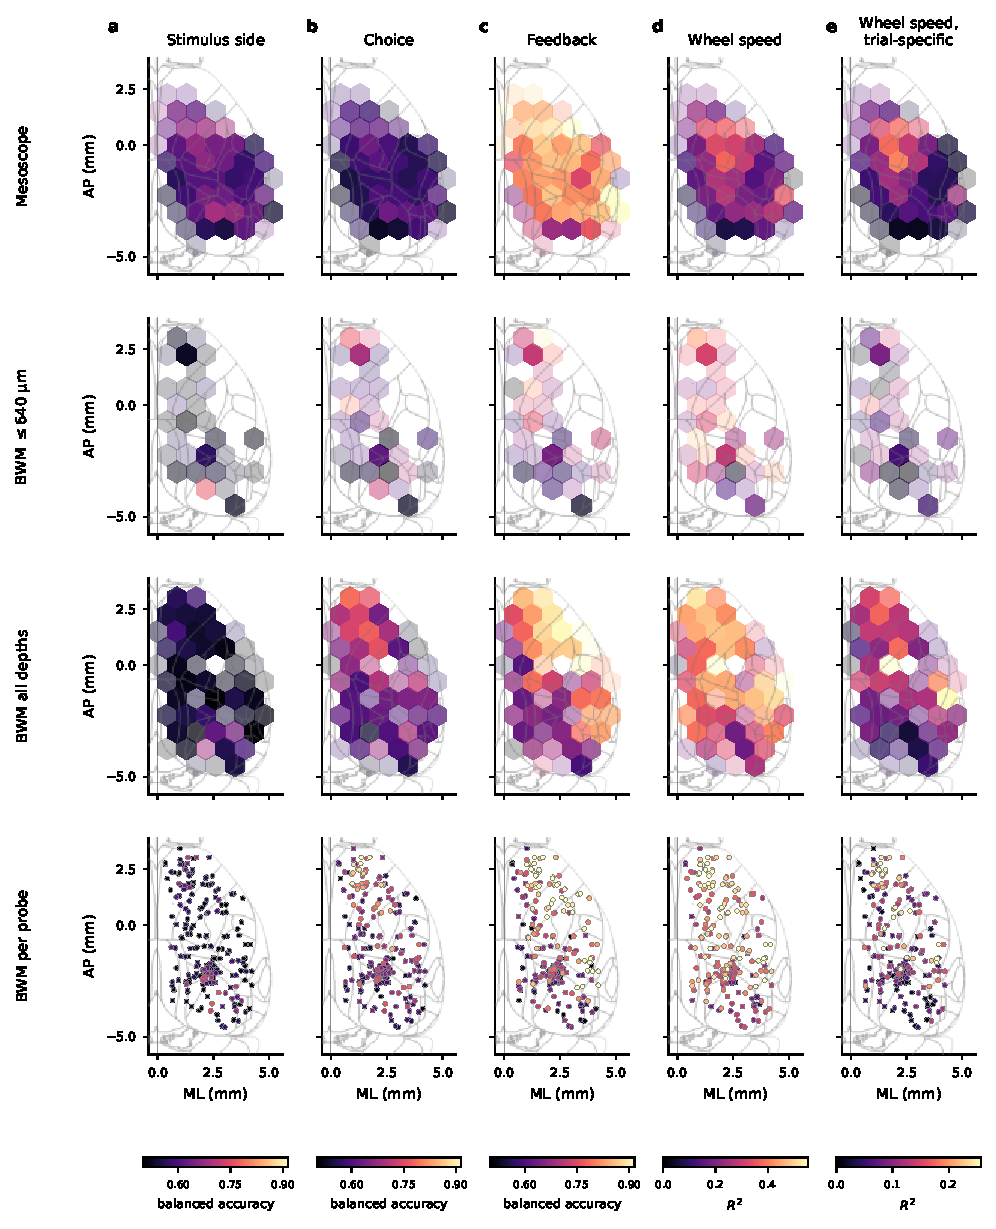
\includegraphics[width=\linewidth,height=0.8\textheight,keepaspectratio]{figures/decoding_all.pdf}
  \caption{\textbf{Decoding from all neurons}. Rows: mesoscope; BWM units within 640\,$\mu$m of the pial surface; BWM at all depths. Each bin (1\,mm hexagon, hemispheres folded) shows the mean over sessions of decoders trained on all neurons of one session in that bin (sessions with $\geq$20 neurons there); mesoscope bins hold far more neurons than BWM bins. Opacity: number of animals (full at $\geq$4). Bottom row: BWM decoded per probe from all its isocortex units at all depths, whichever bins they fall in (209 probes with $\geq$20 units, median 40); each circle sits at the probe's brain entry point (histology-aligned Alyx trajectory, hemispheres folded), higher scores drawn on top where circles overlap; colour scales as in the rows above, so circles beyond the top of a scale saturate. \textbf{a} Stimulus side, balanced accuracy (chance 0.5; colour scale shared by \textbf{a}--\textbf{c}). \textbf{b} Choice. \textbf{c} Feedback. \textbf{d} Wheel speed, cross-validated $R^2$. \textbf{e} Trial-specific wheel speed, $R^2$.}
  \label{fig:decoding_all}
\end{figure}
